\section{Techniques of Circuit Analysis}

\subsection{The Node-Voltage Method}
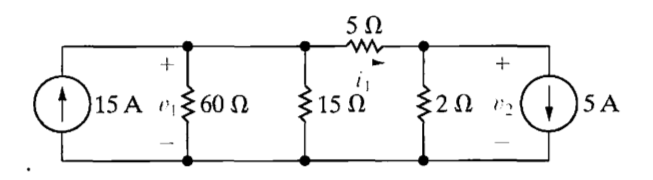
\includegraphics[scale=0.5]{img/c4/p1} \\

\begin{enumerate}
	\item For the circuit shown, use the node-voltage method to find $v_1,v_2, and i_1$
	\item How much power is delivered to the circuit by the 15 A Source?
	\item Repeat 2 for the 5 A source. 
\end{enumerate}

First we can redraw the circuit labeling the node-voltages as follows. 
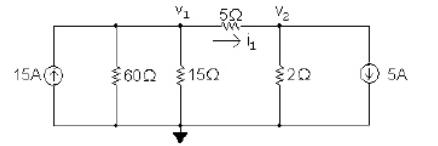
\includegraphics[scale=0.5]{img/c4/a1} \\

The two node voltage equations are:

\begin{align*}
-15 + \frac{v_1}{60} &+  \frac{v_1}{15} &+ \frac{v_1-v_2}{5} &= 0 \\
5 &+ \frac{v_2}{2} &+ \frac{v_2 - v_1}{5} &= 0  \\
\end{align*}

We can then put them into standard form and solve the simultaneous equations:

\begin{align*}
v_1\left(\frac{1}{60} + \frac{1}{15} + \frac{1}{5}\right) &+ v_2(\frac{-1}{5}) &= 15 \\
v_1\left(\frac{-1}{5}\right) &+ v_2\left(\frac{1}{2} + \frac{1}{5}\right) &= -5 \\
\end{align*}

Solving gives us $v_1 = 60 V$ and $v_2 = 10 V$
Which means that:
\begin{align*}
	i_1 &= \frac{v_1 - v_2}{5} \\
	i_1 &= 10A \\
\end{align*}

Next we can solve for the power of the 15 A source as follows:

\begin{align*}
	p_{15A} &= -(15A)v_1 \\
	p_{15A} &= -(15A)(60V) \\ 
	p_{15A} &= -900 W \\
\end{align*}

Which means the source delivers 900 W. 

Finally we can solve for the 5 A source as follows:

\begin{align*}
	p_{5A} &= (5A)v_2 \\
	p_{5A} &= (5A)(10V) \\
	p_{5A} &= 50 W \\
\end{align*}

Which means -50 W is delivered. 

\subsection{The Mesh-Current Method}
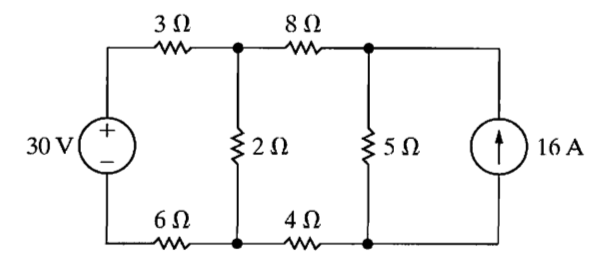
\includegraphics[scale=0.5]{img/c4/p2} \\

For the circuit shown, use the mesh-current method to find the power dissipated in the $2 \Omega$ 
resistor. 

First we redraw the circuit as shown below. \\
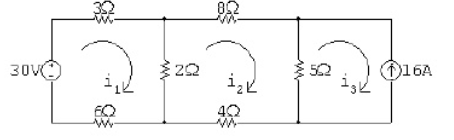
\includegraphics[scale=0.5]{img/c4/a2} \\

Since there is a current source on the far right, we know that $i_3$ is equal to -16A. 
The remaining two mesh equations are:

\begin{align*}
	-30 + 3i_1 + 2(i_1 - i_2) + 6i_1 &= 0 \\
	8i_2 + 5(i_2 + 16) + 4(i_2) + 2(i_2 - i_1) &= 0 \\
\end{align*}

Simplifying gives us:
\begin{align*}
	11i_1 - 2i_2 &= 30 \\
	-2i_1 + 19i_2 &= -80 \\
\end{align*}

Solviing gives us:
\begin{align*}
	i_1 &= 2A \\
	i_2 &= -4A \\
	i_3 &= -16 A \\
\end{align*}

The current in the $2\Omega$ resistor is therefore:\\
$i_1 - i_2 = 6A$ \\
$p_{2\Omega} = (6)^2(2) = 72 W $\\

Thus the $2 \Omega$ resistor dissipates 72 W.


\subsection{Source Transformations}


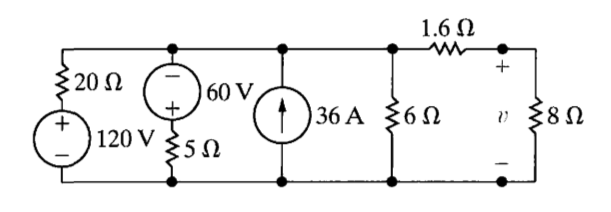
\includegraphics[scale=0.5]{img/c4/p3} \\
Using the above circuit:
\begin{enumerate}
	\item Use a series of source transformations to find the voltage v in the circuit shown.
	\item How much power does the 120 V source deliver to the circuit?
\end{enumerate}

First let's redraw the circuit with voltages and currents labeled:\\
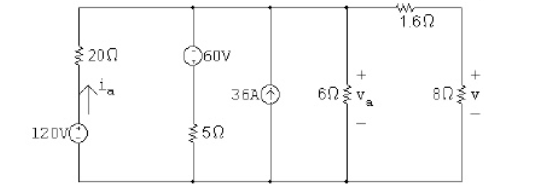
\includegraphics[scale=0.5]{img/c4/a31}\\

Now we can transform the 120 V source in series with the $20\Omega$ resistor into a 6 A source
in parallel with the $20 \Omega$ resistor. Then, transform the -60 V source in series with the
$5 \Omega$ resistor into a -12 A source in parallel with the $5 \Omega$ resistor: \\
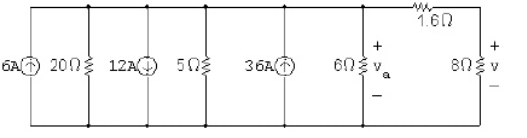
\includegraphics[scale=0.5]{img/c4/a32}\\
Because they are in parallel, we can use KCL to combine the $20\Omega$, $5\Omega$, and 
$6\Omega$ resistors. We can similarly combine the 3 current sources. This is shown below:
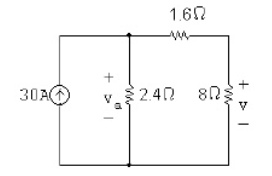
\includegraphics[scale=0.5]{img/c4/a33}\\
Next, we can combine the resulting current source with the $2.4\Omega$ resistor into a 72 V source
in series with a $2.4\Omega$ resistor, which can then be added to the $1.6\Omega$ resistor. This
is shown below:\\
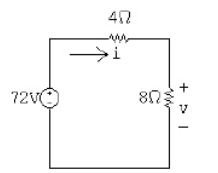
\includegraphics[scale=0.5]{img/c4/a34}\\
Now we can use voltage division to calcuate $v$:\\
$v = \frac{8}{12} \times 72 = 48 V$

We can use the last circuit to calculate $i$: \\
$ i = \frac{v}{8} = \frac{48}{8} = 6A $ \\

Now we can use $i$ to calculate $v_a$ in the circuit on the left:
\\$ v_a = 6(1.6 + 8) = 57.6 V $ \\
We can see in the original equation that $v_a$ is also the voltage drop across the series
combination of 120V and $20\Omega$

\subsection{Thevenin's and Norton's Equivalents}

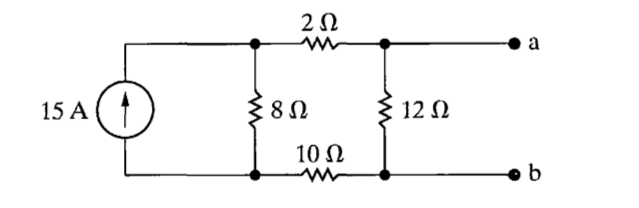
\includegraphics[scale=0.5]{img/c4/p4} \\
Find the Norton Equivalent circuit with respect to terminals a and b.
To solve the problem follow the below steps:
\begin{enumerate}
	\item Perform a source transformation turning 15 A source and $8\Omega$ resistor into 
	a series combination of 120 V and $8\Omega$ resistor. See the first circuit below. 
	\item Combine the $2\Omega$, $8\Omega$, and $10\Omega$ resistors in series to get
	$20 \Omega$
	\item Combine the $20\Omega$ resistor and 120 V source into a parallel combination
	of 6 A source and $20\Omega$ resistor. This is shown in the second circuit below.
	\item Combine the $20\Omega$ and $12\Omega$ parallel resistors to give $7.5\Omega$.
\end{enumerate}

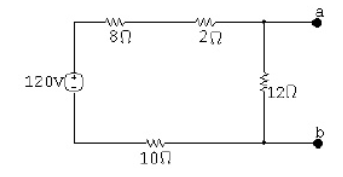
\includegraphics[scale=0.5]{img/c4/a41} \\
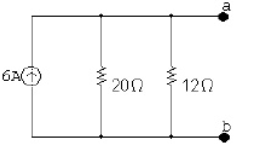
\includegraphics[scale=0.5]{img/c4/a42} \\

Thus the Norton equivalent is a 6A source and a $7.5\Omega$ Resistor. 

\subsection {Maximum Power Transfer}

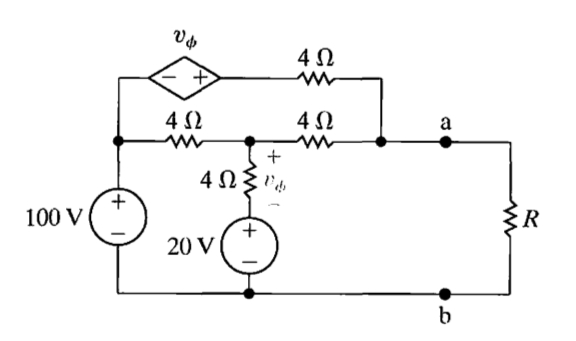
\includegraphics[scale=0.5]{img/c4/p5} \\
\begin{enumerate}
	\item Find the value of $R$ that enables the circuit shown to deliver maximum power
	to the terminals a and b.
	\item Find the maximum power delivered to R. 
\end{enumerate}

First we find the Thevenin equivalent circuit. To find $v_{TH}$ we create an open circuit
between a and b and use the node voltage method to solve: \\
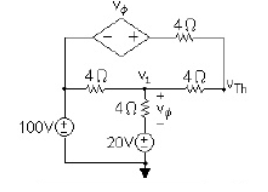
\includegraphics{img/c4/a51} \\
\begin{align*}
	0 &= \frac{v_{th} - (100 + v_{\phi})}{4} + {v_{th} - v_1}{4} \\
	0 &= \frac{v_1 -100}{4} + \frac{v_1-20}{4} + \frac{v_1 -v_{th}}{4} \\
\end{align*}

The dependent source is: \\
$v_{\phi} = v_1 - 20$ \\

Putting the three equations together we get:
\begin{align*}
	v_{th}\left( \frac{1}{4} + \frac{1}{4}  \right) &+ v_1\left( \frac{-1}{4} \right) &+ v_{phi} \left( \frac{-1}{4} \right) &= 25 \\
	v_{th}\left( \frac{-1}{4} \right) &+ v_1 \left( \frac{1}{4} + \frac{1}{4} + \frac{1}{4} \right) &+ v_{\phi}(0) &= 30 \\
	v_{th}(0) &+ v_1(1) &+ v_{\phi}(-1) &= 20 \\
\end{align*}

Solving for all three equations gives us:
\begin{align*}
	v_{th} &= 120 V \\
	v_1 &= 80 V \\
	v_{\phi} &= 60 V \\	
\end{align*}

Now we create a short circuit between nodes a and b and use the mesh current method: \\
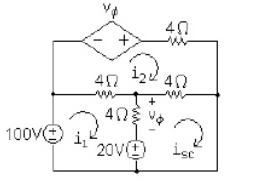
\includegraphics{img/c4/a52} \\

The mesh current equations are: \\
\begin{align*}
	0 &= -100 + 4(i_1 - i_2) + v_{\phi} + 20 \\
	0 &= -v_{\phi} + 4i_2 + 4(i_2 -i_{sc}) + 4(i_2 - i_1) \\
	0 &= -20 - v_{\phi} + 4 (i_{sc} - i_2) \\
\end{align*}

The dependent source equation is: \\
$ v_{\phi} = 4(i_1 - i_{sc}) $ \\
Putting the four equation together gives:\\

\begin{align*}
	4i_1 - 4i_2 + 0i_{sc} + v_{\phi} &= 80 \\
	-4i_1 +12i_2 - 4i_{sc} + v_{\phi} &= 0 \\
	0i_1 - 4i_2 + 4i_{sc} - v_{\phi} &= 20 \\
	4i_1 + 0i_2 - 4i_{sc} - v_{\phi} &= 0 \\
\end{align*}

Solving gives:
\begin{align*}
	i_1 &= 45 A \\
	i_2 &= 30 A \\
	i_{sc} &= 40 A \\
	v_{\phi} &= 20 V \\
\end{align*}

Then: \\
$ R_{TH} = \frac{v_{TH}}{i_{sc}} = \frac{120}{40} = 3 \Omega $\\

For maximum power transfer, $R = R_{TH} = 3\Omega $  

The Thevenin voltage voltage, $v_{TH} = 120 V$, splits equally between the Thevenin resistance
and the load resistance so: 
\\ $v_{load} = \frac{120}{2} = 60 V $ \\
\\ $p_{max} = \frac{v^2_{load}}{R_{load}} = \frac{60^2}{3} = 1200 W $ \\

\subsection {Superposition}



